\section{Virtual Organization Over NDN}

\begin{figure*}[t]
  \centering
  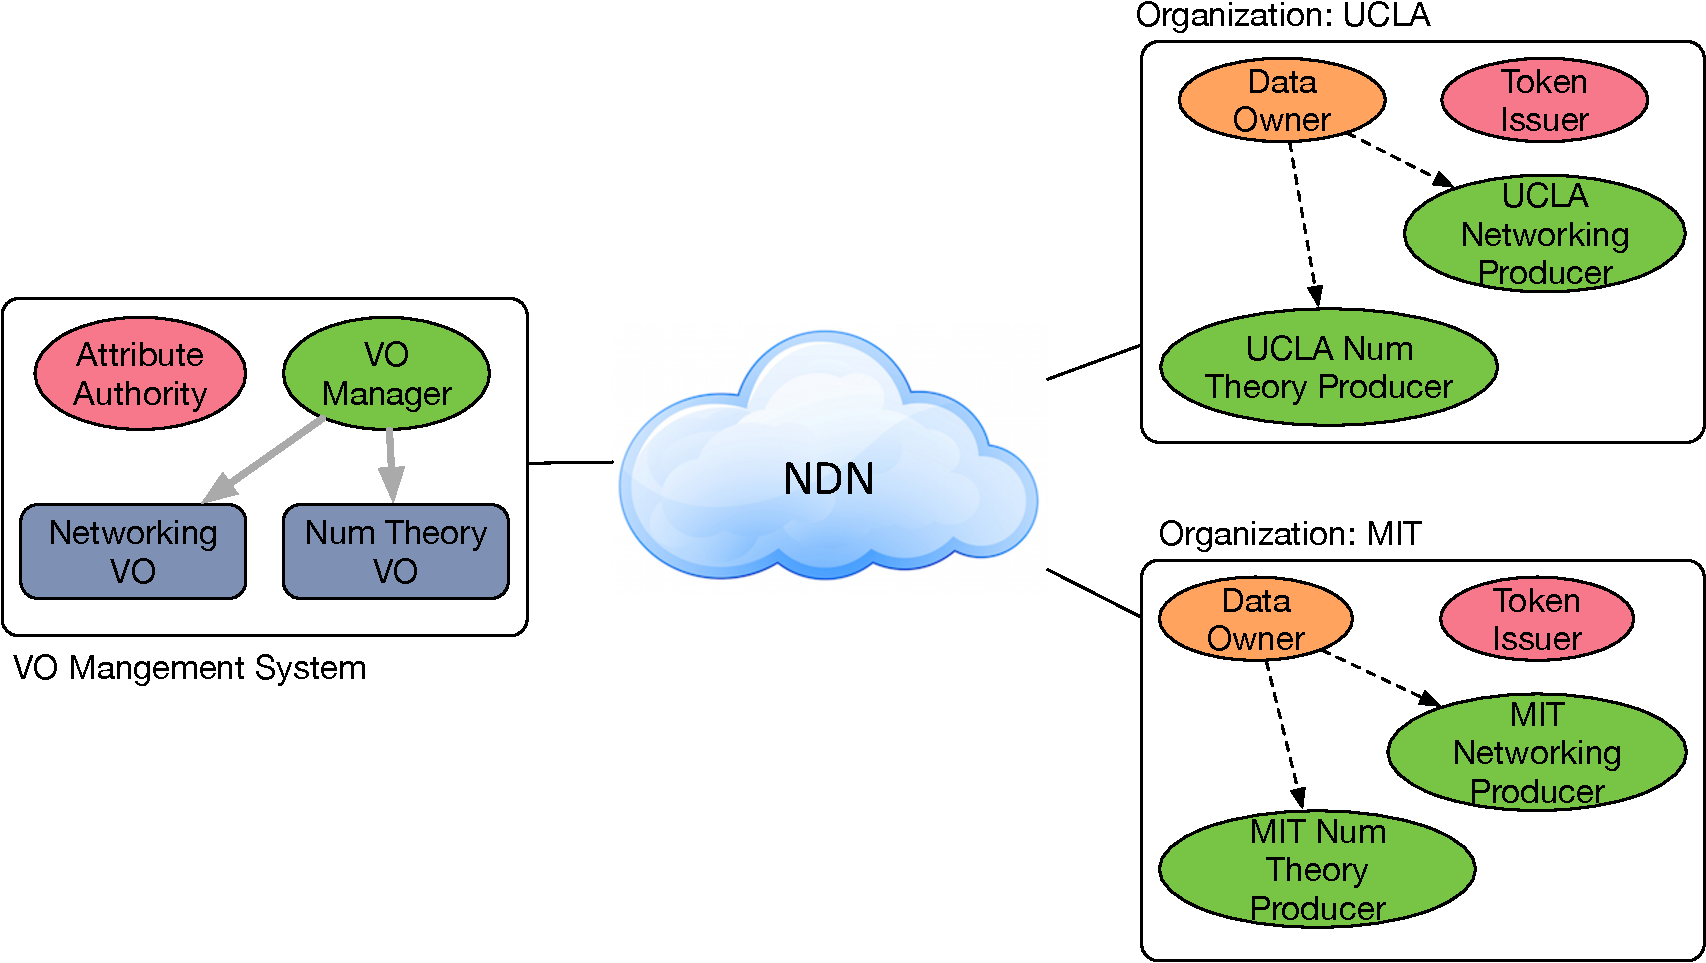
\includegraphics[scale=0.5]{figures/example}
  \vspace{-3mm}
  \caption{An example of how VO system work}
  \label{fig:example}
\end{figure*}

To facilitate explanation, in this section, we will use the following example (\ref{fig:example}) to illustrate the VO system.
The right side is the VO management system, which contains an \textbf{attribute authority} and a \textbf{VO manager}.
Attribute authority will setup the CPABE environment by generating public parameters and a secret master key.
The VO manager will create the VO, the data packet(s) containing the name category.
Both UCLA and MIT will produce networking lecture data and Number-theory lecture data.
There are two real-world organizations in our example: UCLA and MIT.
Besides producers which are the green circles, each organization also contains one \textbf{data owner} and one \textbf{token issuer}.
Data owner is the one who define the access rules for producer.
Token issuer takes the duty to help attribute authority to verify consumer's identity.

In NDN, each party is supposed to have an identity.
To make the example clear, we have the name like:

\begin{verbatim}
VO attribute authority: /vo/authority
VO manager: /vo/manager

UCLA token issuer: /ucla/token-issuer
UCLA data owner: /ucla/data-owner
UCLA network producer: /ucla/network
UCLA number theory producer: /ucla/num-theory
\end{verbatim}

In our example, there are also two VOs containing networking lecture data names and number theory lecture data names respectively.
In this way, the authorised consumers could easily access the networking/number theory lecture data both from UCLA and MIT through VO.

\subsection{VO Mangement System}

VO management system mainly contains two parts: attribute authority and VO manager.
The attribute authority will take the duty to setup the CPABE environment and issue decryption key for authorised consumers.
The VO manager will collect data information from each organization and produce VOs.

\subsubsection{Attribute Authority}
The attribute authority (AA) is a globally trust anchor.
All parties, no matter producer or consumer, should all trust the authority.
However, the existence of attribute authority won't lower down the security of the whole system and attribute authority won't become the single point of failure when system is running.
In the VO system, the attribute authority only works at the preliminary phase.
Once finish the system setup, the attribute authority should go offline to avoid potential attack from outside.

Before the system start running, AA would generate the public parameters which is a data packet and a secret master key.
In our system, the public parameter has the naming convention \texttt{/[AA-prefix]/PUB/<timestamp>}.
For instance, in the example, a possible name can be \texttt{/vo/authority/PUB/201706151200}.
The public parameters data packet will be signed by VO management system's certificate.
Regarding the master key, once the secret master key get compromised, the system will be broken.
In the preliminary phase, the authority will also issue consumer's decryption key based on the information provided by the token issuer.
The detail will be illustrated in the section \ref{token-issuer}.
This makes sure that the AA will only talk with trusted parties during the preliminary phase.

Once the system starts running, the AA should go offline immediately.
In the future, the AA should be awaken only when consumer's key get compromised and when there are new attributes.
Notice, even when AA is working, AA only needs to talk with token issuer, which is trusted.
If the token issuer corrupts, there is no security in system; thus only trustworthy party, like universities, government departement and etc., can become token issuer.

\subsubsection{VO Manager}
VO manager is the service provider who define the name category and produce VO packets.
All the organizations who wants to join the VO are supposed to provide the data information for VO manager.
The information should at least contains the data name and a category suggestion.
VO manager can use the application-readable data name to put each name into one or more VOs.

To protect the category information from unauthorized users, the data content should be encrypted by specific attribute.
In our system, there are VO attributes: "VO-001", "VO-002" and etc.
This kind of attribute is used to encrypt the name category.
Only user who has the corresponding key could see the category.
Notice that even users can see the category, it does not mean that users could consume the data for the data packets are encrypted by organization's policies.
For instance, assume the network lecture VO's data name is \texttt{/ucla/network/lesson1}

Each VO data packet

\subsection{Organization}

\subsubsection{Producer}

\subsubsection{Data Owner}

\subsubsection{Token Issuer} \label{token-issuer}


\subsection{Consumer}